\chapter{Introduction}
\label{introduction}
A finite automaton (FA) is a model of computation with applications in different branches of computer science, e.g., compiler design, formal verification, 
designing of digital circuits or natural language processing. In formal verification alone are its uses abundant, 
for example in model checking of safety temporal properties, abstract regular model checking \cite{armc}, static analysis \cite{metal}, 
or decision procedures of some logics, such as Presburger arithmetic or weak 
monadic second-order theory of one successor (WS1S) \cite{mona}.

Many of the mentioned applications need to perform certain expensive operations on FA, such as checking universality of an FA (i.e., checking whether it
accepts any word over a given alphabet), or checking language inclusion of a pair of FA (i.e., testing whether the language of one FA is a subset of the language
of the second FA). The Classical (so called \emph{textbook}) approach is based on \emph{complementation} of the language of an FA. Complementation is easy for 
\emph{deterministic} FA (DFA)--just swapping accepting and non-accepting states--but a hard problem for \emph{nondeterministic} FA (NFA), which need 
to be determinised first (this may lead to an exponential explosion in the number of the states of the automaton). 
Both operations of checking of universality and language inclusion over NFA are PSPACE-complete problems \cite{cav06}.

Recently, there has been a considerable advance in techniques for dealing with these problems. The new techniques are either based on the so-called 
\emph{antichains} \cite{cav06,tacas10} or the so-called \emph{bisimulation up to congruence} \cite{popl13}. 
In general, those techniques do not need an explicit construction of the complement
automaton. They only construct a sub-automaton which is sufficient for either proving that the universality or inclusion hold, or finding a counterexample.

Unfortunately, there is currently no efficient implementation of a general NFA library that would use the state-of-the-art algorithms for the mentioned
operations on automata. The
closest implementation is VATA \cite{libvata}, a general library for nondeterministic finite \emph{tree} automata, which can be used even for NFA (being modelled 
as unary tree automata) but not with the optimal performance given by its overhead that comes with the ability to handle much richer structures. 
 
The goal of this work is two-fold: (i) extending VATA with an NFA module implementing basic operations on NFA, such as union, intersection, or 
checking language inclusion, and (ii) an efficient design and implementation of checking language inclusion of NFA using 
bisimulation up to congruence (which is missing in VATA for tree automata).

After this introduction, in the \ref{teorie}nd chapter of this document, 
will be defined theoretical background. The \ref{chapInclusion}rd chapter will describe efficient approaches to language inclusion testing.
Existing libraries for finite automata manipulation and the VATA library will be introduced in chapter \ref{libraries}. 
Design of extension for VATA 
will take place in chapter \ref{arch}. Implementation and optimization is possible to find in chapter \ref{implementation}. Evaluation will be
described in chapter \ref{eval} and final conclusion in chapter \ref{concl}.


\chapter{Preliminaries}
This chapter contains theoretical fundations of the thesis. No proofs are given, because they can be found in literature. 
First, the languages will be defined, then finite automata and their context, the regular languages and their closure properties. 
\label{teorie}

\section{Languages}
We call a finite set of symbols $\Sigma$ an \emph{alphabet}. A~\emph{word} $w$ over $\Sigma$ of \emph{length} $n$ is a finite sequence of symbols 
$w=a_1\ldots a_n$, where $\forall 1 \leq i \leq n\ . \ a_i \in \Sigma$. An \emph{empty word} is denoted as $\epsilon \not\in\Sigma$ and its length is $0$. 
We define \emph{concatenation} as an associative binary operation on words over $\Sigma$ represented by the symbol $\cdot$ such that for two words $u=a_1\ldots a_2$
and $v=b_1\ldots b_n$ over $\Sigma$ it holds that $\epsilon\cdot u=u\cdot\epsilon=u$ and $u\cdot v=a_1 \ldots a_nb_1 \ldots b_m$.
We define a symbol $\Sigma^{*}$ as a set of all words over $\Sigma$ including the empty word and a symbol $\Sigma^{+}$ as a set of 
all words over $\Sigma$ without the empty word, 
so it holds that $\Sigma_{*}=\Sigma_{+}\cup\epsilon$. A~\emph{language} $L$ over $\Sigma$ is a subset of $\Sigma^{*}$.
Given a pair of languages $L_1$ over an alphabet $\Sigma_{1}$ and $L_{2}$ over an alphabet $\Sigma_{2}$. Their concatenation is defined by 
$L_1\cdot L_2=\{x\cdot y\ |\ x\in L_1, y\in L_2 \}$.
We define \emph{iteration} $L^{*}$ and \emph{positive} iteration $L^{+}$ of a language $L$ over an alphabet $\Sigma$ \emph{iteration} as:
	\begin{itemize}
		\item $L^0=\{\epsilon\}$
		\item $L^{n+1}=L\cdot L^n$, for $n \leq 1$
    \item $L^{*}=\bigcup_{n\leq 0} L^{n}$
    \item $L^{+}=\bigcup_{n\leq 1} L^{n}$
	\end{itemize}

\section{Finite Automata}
\label{defFA}

	\subsection{Nondeterministic Finite Automaton}
	\label{defNFA}
		\emph{A Nondeterministic Finite Automaton} (NFA) is a quintuple $\mathcal{A}=(Q,\Sigma,\delta,I,F)$, where
		\begin{itemize}
			\item $Q$ is a finite set of states,
			\item $\Sigma$ is an alphabet,
			\item $\delta \subseteq Q \times \Sigma \times Q$ is a transition relation. We use $p \xrightarrow{a} q$ to denote that $(p,a,q)\in\delta$,
			\item $I$ is finite set of states, that $I \subseteq Q$. Elements of $I$ are called initial states.
			\item $F$ is finite set of states, that $F \subseteq Q$. Elements of $F$ are called final states.
		\end{itemize}

    An example of an NFA is shown on the picture \label{pic_ex_nfa}.
%%%%example of NFA
		\begin{figure}[h]
		\begin{center}
		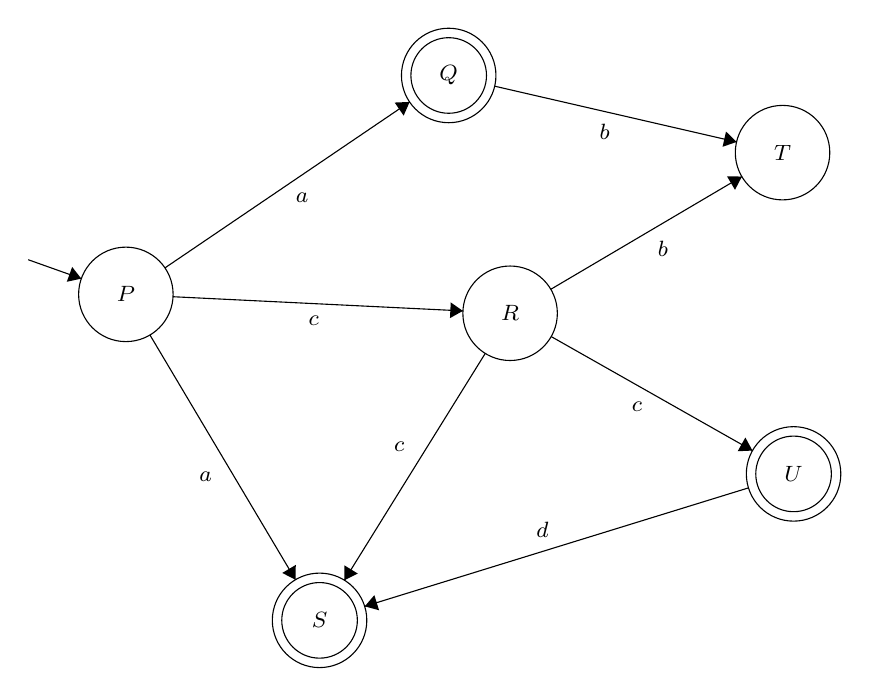
\begin{tikzpicture}[scale=0.2]
				\tikzstyle{every node}+=[inner sep=0pt]
				\draw [black] (9.4,-29.6) circle (3);
				\draw (9.4,-29.6) node {$P$};
				\draw [black] (29.9,-15.7) circle (3);
				\draw (29.9,-15.7) node {$Q$};
				\draw [black] (29.9,-15.7) circle (2.4);
				\draw [black] (33.8,-30.8) circle (3);
				\draw (33.8,-30.8) node {$R$};
				\draw [black] (21.7,-50.3) circle (3);
				\draw (21.7,-50.3) node {$S$};
				\draw [black] (21.7,-50.3) circle (2.4);
				\draw [black] (51.1,-20.6) circle (3);
				\draw (51.1,-20.6) node {$T$};
				\draw [black] (51.8,-41) circle (3);
				\draw (51.8,-41) node {$U$};
				\draw [black] (51.8,-41) circle (2.4);
				\draw [black] (3.2,-27.4) -- (6.57,-28.6);
				\fill [black] (6.57,-28.6) -- (5.99,-27.86) -- (5.65,-28.8);
				\draw [black] (11.88,-27.92) -- (27.42,-17.38);
				\fill [black] (27.42,-17.38) -- (26.47,-17.42) -- (27.04,-18.25);
				\draw (20.6,-23.15) node [below] {$a$};
				\draw [black] (10.93,-32.18) -- (20.17,-47.72);
				\fill [black] (20.17,-47.72) -- (20.19,-46.78) -- (19.33,-47.29);
				\draw (14.9,-41.21) node [left] {$a$};
				\draw [black] (12.4,-29.75) -- (30.8,-30.65);
				\fill [black] (30.8,-30.65) -- (30.03,-30.11) -- (29.98,-31.11);
				\draw (21.33,-30.95) node [below] {$c$};
				\draw [black] (32.82,-16.38) -- (48.18,-19.92);
				\fill [black] (48.18,-19.92) -- (47.51,-19.26) -- (47.29,-20.23);
				\draw (39.8,-18.73) node [below] {$b$};
				\draw [black] (36.38,-29.28) -- (48.52,-22.12);
				\fill [black] (48.52,-22.12) -- (47.57,-22.1) -- (48.08,-22.96);
				\draw (43.5,-26.2) node [below] {$b$};
				\draw [black] (36.41,-32.28) -- (49.19,-39.52);
				\fill [black] (49.19,-39.52) -- (48.74,-38.69) -- (48.25,-39.56);
				\draw (41.85,-36.4) node [below] {$c$};
				\draw [black] (48.93,-41.89) -- (24.57,-49.41);
				\fill [black] (24.57,-49.41) -- (25.48,-49.66) -- (25.18,-48.7);
				\draw (35.85,-45.1) node [above] {$d$};
				\draw [black] (32.22,-33.35) -- (23.28,-47.75);
				\fill [black] (23.28,-47.75) -- (24.13,-47.33) -- (23.28,-46.81);
				\draw (27.12,-39.26) node [left] {$c$};
				\end{tikzpicture}
			\end{center}
      \label{pic_ex_nfa}
			\caption{An example of a NFA}
			\end{figure}
%%%end of nfa picture



	\subsection{Deterministic Finite Automaton}
	\label{defDFA}
  A~\emph{deterministic finite automaton} (DFA) is a special case of an NFA, where $\delta$ is a partial function 
$\delta: Q\times \Sigma \to Q$ and $|I| \leq 1$. To be precise, we give the whole definition of DFA.\newline
\newline
		A DFA is a quintuple $\mathcal{A}=(Q,\Sigma,\delta,I,F)$ where
		\begin{itemize}
			\item $Q$ is a finite set of states,
			\item $\Sigma$ is  an alphabet,
			\item $\delta$:  $Q \times \Sigma \to Q$ is a partial transition function. We use $p \xrightarrow{a} q$ to denote that $\delta(p,a)=q$
			\item $I\subseteq Q$ is finite set of initial states, that $|I| \leq 1$.
			\item $F\subseteq Q$ is finite set of final states.
		\end{itemize}
    An example of a DFA is given on the picture \ref{pic_ex_dfa}.


%%%example of DFA
\begin{figure}[h]
\begin{center}
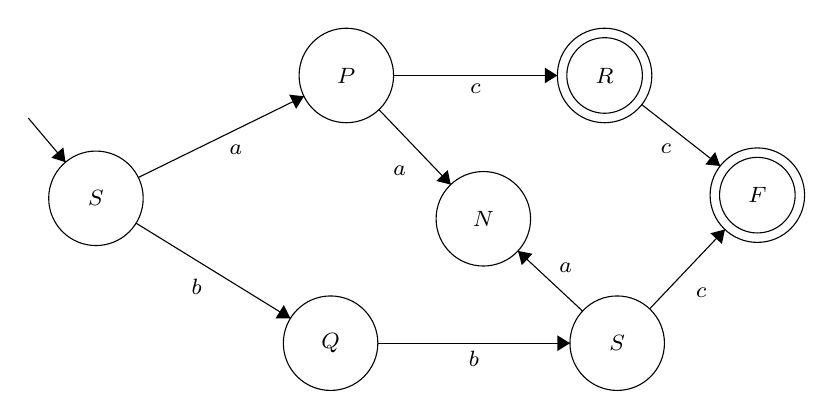
\begin{tikzpicture}[scale=0.2]
\tikzstyle{every node}+=[inner sep=0pt]
\draw [black] (9.9,-28) circle (3);
\draw (9.9,-28) node {$S$};
\draw [black] (25.8,-20.2) circle (3);
\draw (25.8,-20.2) node {$P$};
\draw [black] (24.8,-37.2) circle (3);
\draw (24.8,-37.2) node {$Q$};
\draw [black] (42.2,-20.2) circle (3);
\draw (42.2,-20.2) node {$R$};
\draw [black] (42.2,-20.2) circle (2.4);
\draw [black] (43,-37.2) circle (3);
\draw (43,-37.2) node {$S$};
\draw [black] (51.9,-27.8) circle (3);
\draw (51.9,-27.8) node {$F$};
\draw [black] (51.9,-27.8) circle (2.4);
\draw [black] (34.5,-29.3) circle (3);
\draw (34.5,-29.3) node {$N$};
\draw [black] (5.6,-22.9) -- (7.97,-25.71);
\fill [black] (7.97,-25.71) -- (7.83,-24.77) -- (7.07,-25.42);
\draw [black] (12.59,-26.68) -- (23.11,-21.52);
\fill [black] (23.11,-21.52) -- (22.17,-21.42) -- (22.61,-22.32);
\draw (18.79,-24.6) node [below] {$a$};
\draw [black] (12.45,-29.58) -- (22.25,-35.62);
\fill [black] (22.25,-35.62) -- (21.83,-34.78) -- (21.3,-35.63);
\draw (16.3,-33.1) node [below] {$b$};
\draw [black] (28.8,-20.2) -- (39.2,-20.2);
\fill [black] (39.2,-20.2) -- (38.4,-19.7) -- (38.4,-20.7);
\draw (34,-20.7) node [below] {$c$};
\draw [black] (27.8,-37.2) -- (40,-37.2);
\fill [black] (40,-37.2) -- (39.2,-36.7) -- (39.2,-37.7);
\draw (33.9,-37.7) node [below] {$b$};
\draw [black] (45.06,-35.02) -- (49.84,-29.98);
\fill [black] (49.84,-29.98) -- (48.92,-30.22) -- (49.65,-30.9);
\draw (47.98,-33.97) node [right] {$c$};
\draw [black] (44.56,-22.05) -- (49.54,-25.95);
\fill [black] (49.54,-25.95) -- (49.22,-25.06) -- (48.6,-25.85);
\draw (46.09,-24.5) node [below] {$c$};
\draw [black] (27.87,-22.37) -- (32.43,-27.13);
\fill [black] (32.43,-27.13) -- (32.24,-26.21) -- (31.51,-26.9);
\draw (29.62,-26.22) node [left] {$a$};
\draw [black] (40.8,-35.16) -- (36.7,-31.34);
\fill [black] (36.7,-31.34) -- (36.94,-32.25) -- (37.62,-31.52);
\draw (39.72,-32.76) node [above] {$a$};
\end{tikzpicture}
\end{center}
\caption{An example of a DFA}
\label{pic_ex_dfa}
\end{figure}
%%%%end of DFA example

%%%comment
\begin{comment}
	\subsection{Function $\hat{\delta}$}
	\label{defFunct}
		\begin{definition}
		A function $\hat{\delta}$ is define as
		\begin{description}
			$\hat{\delta}: Q\times\Sigma^{*}\rightarrow Q$
		\end{description}

		from $\delta$ by induction on the length of $x$:
			\begin{itemize}
				\item $\hat{\delta}(q,\epsilon)=q$, where $\epsilon$ is empty string
				\item $\hat{\delta}(q,xa)=\delta(\hat{\delta}(q,x),a)$
			\end{itemize}
		\end{definition}
\end{comment}
%%%%		


  \subsection{Operations over Finite Automata}
    \subsubsection{Automata Union}
    \label{defAUnion}
      Given a pair of NFA $\mathcal{A}=(Q_\mathcal{A},\Sigma,\delta_\mathcal{A},I_\mathcal{A},F_\mathcal{A})$ 
      and $\mathcal{B}=(Q_\mathcal{B},\Sigma,\delta_\mathcal{B},I_\mathcal{B},F_\mathcal{B})$. Their union is defined by
      \begin{description}
        \item $A \cup B=(Q_\mathcal{A}\cup Q_\mathcal{B},\Sigma,
            \delta_\mathcal{A}\cup\delta_\mathcal{B},I_\mathcal{A}\cup I_\mathcal{B},F_\mathcal{A}\cup F_\mathcal{B})$
      \end{description}
    
    \subsubsection{Automata Intersection}
    \label{defAInter}
      Given a pair of NFA, $A=(Q_\mathcal{A},\Sigma,\delta_\mathcal{A},I_\mathcal{A},F_\mathcal{A})$ 
      and $B=(Q_\mathcal{B},\Sigma,\delta_\mathcal{B},I_\mathcal{B},F_\mathcal{B})$. Their intersection is defined by
      \begin{description}
        \item $A \cap B=(Q_\mathcal{A}\cap Q_\mathcal{B},\Sigma,\delta,I_\mathcal{A}\cap I_\mathcal{B},F_\mathcal{A}\cap F_\mathcal{B})$\
      \end{description}
      where $\delta$ is defined by
      \begin{description}
        \item $\delta = 
        \{(p_1,q_1) \xrightarrow{a} (p_2,q_2)\ |\ p_1 \xrightarrow{a} p_2 \in \delta_\mathcal{A} \wedge q_1 \xrightarrow{a} q_2 \in \delta_\mathcal{B})\}$\
      \end{description}

      \subsubsection{Automata Product}
      \label{defAutProd}
      Given a pair of NFA, $A=(Q_\mathcal{A},\Sigma,\delta_\mathcal{A},I_\mathcal{A},F_\mathcal{A})$ 
      and $B=(Q_\mathcal{B},\Sigma,\delta_\mathcal{B},I_\mathcal{B},F_\mathcal{B})$. Their product is defined by
      \begin{description}
        \item $A \times B=(Q_\mathcal{A}\times Q_\mathcal{B},\Sigma,\delta,I_\mathcal{A}\times I_\mathcal{B},F_\mathcal{A}\times F_\mathcal{B})$\
      \end{description}
      where $\delta$ is defined by
      \begin{description}
        \item $\delta = 
        \{(p_1,q_1) \xrightarrow{a} (p_2,q_2)\ |\ p_1 \xrightarrow{a} p_2 \in \delta_\mathcal{A} \wedge q_1 \xrightarrow{a} q_2 \in \delta_\mathcal{B})\}$\
      \end{description}

  \subsubsection{Subset construction}
	\label{subset}
	Now we will define how to construct equivalent DFA $\mathcal{A}_{det}$ for a given NFA $\mathcal{A}=(Q,\Sigma,\delta,S,F)$. 
  \newline
  \newline
	\label{defSubset}
	$\mathcal{A}_{det}=(2^Q,\Sigma,\delta_{det},S,F_{det})$, where
	\begin{itemize}
		\item $2^Q$ is power set of $Q$
		\item $F_{det}=\{Q'\subseteq Q\ |\ Q'\cap F \not = \varnothing\}$
		\item $\delta_{det}(Q',a)=\bigcup\limits_{q\in Q'}\delta(q,a)$, where $a\in\Sigma$
	\end{itemize}

  This classical ("textbook") approach is called \emph{subset construction}.
    An example of this approach is shown on the picutre \ref{pic_sub}.
	
	%%%%example of NFA to DFA	
	\begin{figure}[h]
\begin{center}
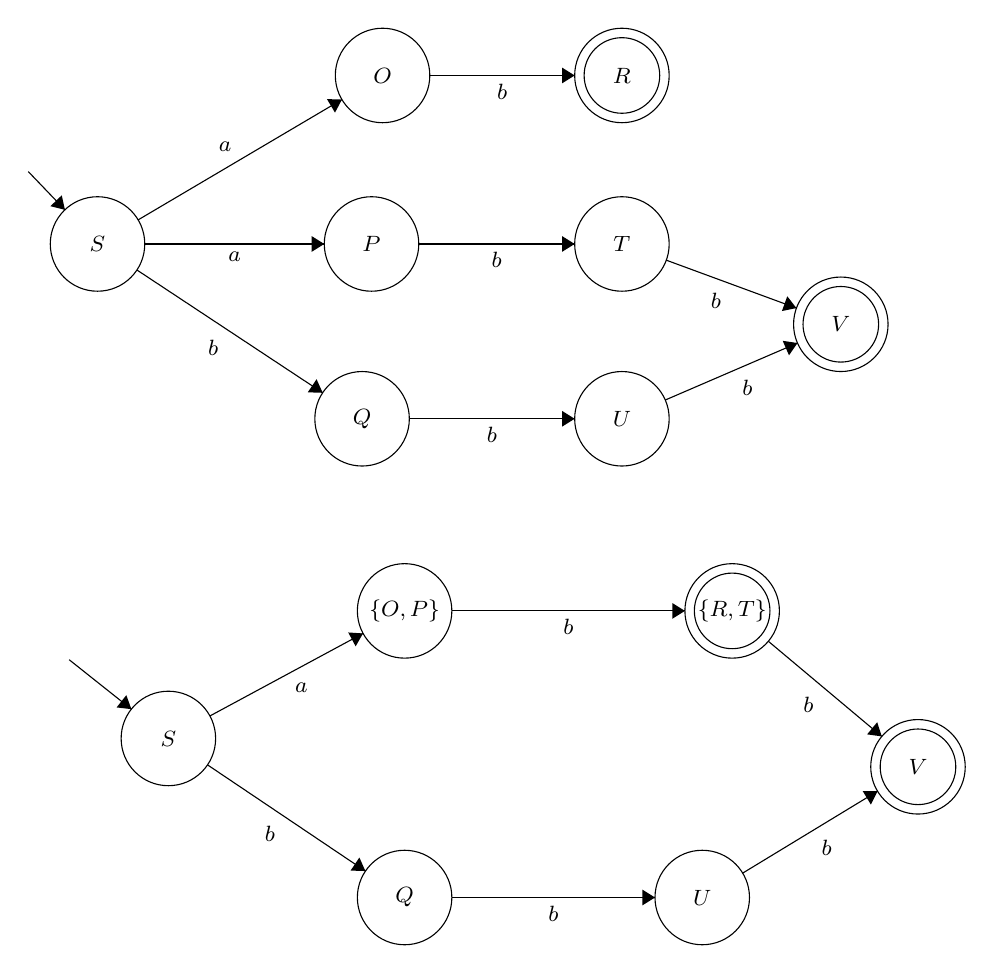
\begin{tikzpicture}[scale=0.2]
\tikzstyle{every node}+=[inner sep=0pt]
\draw [black] (7.9,-14.8) circle (3);
\draw (7.9,-14.8) node {$S$};
\draw [black] (26,-4.1) circle (3);
\draw (26,-4.1) node {$O$};
\draw [black] (25.3,-14.8) circle (3);
\draw (25.3,-14.8) node {$P$};
\draw [black] (24.7,-25.9) circle (3);
\draw (24.7,-25.9) node {$Q$};
\draw [black] (41.2,-4.1) circle (3);
\draw (41.2,-4.1) node {$R$};
\draw [black] (41.2,-4.1) circle (2.4);
\draw [black] (41.2,-14.8) circle (3);
\draw (41.2,-14.8) node {$T$};
\draw [black] (41.2,-25.9) circle (3);
\draw (41.2,-25.9) node {$U$};
\draw [black] (55.1,-19.9) circle (3);
\draw (55.1,-19.9) node {$V$};
\draw [black] (55.1,-19.9) circle (2.4);
\draw [black] (12.4,-46.2) circle (3);
\draw (12.4,-46.2) node {$S$};
\draw [black] (27.4,-38.1) circle (3);
\draw (27.4,-38.1) node {$\{O,P\}$};
\draw [black] (27.4,-56.3) circle (3);
\draw (27.4,-56.3) node {$Q$};
\draw [black] (48.2,-38.1) circle (3);
\draw (48.2,-38.1) node {$\{R,T\}$};
\draw [black] (48.2,-38.1) circle (2.4);
\draw [black] (46.3,-56.3) circle (3);
\draw (46.3,-56.3) node {$U$};
\draw [black] (60,-48) circle (3);
\draw (60,-48) node {$V$};
\draw [black] (60,-48) circle (2.4);
\draw [black] (3.5,-10.2) -- (5.83,-12.63);
\fill [black] (5.83,-12.63) -- (5.63,-11.71) -- (4.91,-12.4);
\draw [black] (10.48,-13.27) -- (23.42,-5.63);
\fill [black] (23.42,-5.63) -- (22.47,-5.6) -- (22.98,-6.46);
\draw (16,-8.95) node [above] {$a$};
\draw [black] (10.9,-14.8) -- (22.3,-14.8);
\fill [black] (22.3,-14.8) -- (21.5,-14.3) -- (21.5,-15.3);
\draw (16.6,-15.3) node [below] {$a$};
\draw [black] (10.4,-16.45) -- (22.2,-24.25);
\fill [black] (22.2,-24.25) -- (21.81,-23.39) -- (21.25,-24.22);
\draw (15.25,-20.85) node [below] {$b$};
\draw [black] (29,-4.1) -- (38.2,-4.1);
\fill [black] (38.2,-4.1) -- (37.4,-3.6) -- (37.4,-4.6);
\draw (33.6,-4.6) node [below] {$b$};
\draw [black] (28.3,-14.8) -- (38.2,-14.8);
\fill [black] (38.2,-14.8) -- (37.4,-14.3) -- (37.4,-15.3);
\draw (33.25,-15.3) node [below] {$b$};
\draw [black] (27.7,-25.9) -- (38.2,-25.9);
\fill [black] (38.2,-25.9) -- (37.4,-25.4) -- (37.4,-26.4);
\draw (32.95,-26.4) node [below] {$b$};
\draw [black] (43.95,-24.71) -- (52.35,-21.09);
\fill [black] (52.35,-21.09) -- (51.41,-20.95) -- (51.81,-21.87);
\draw (49.17,-23.41) node [below] {$b$};
\draw [black] (44.02,-15.83) -- (52.28,-18.87);
\fill [black] (52.28,-18.87) -- (51.7,-18.12) -- (51.36,-19.06);
\draw (47.17,-17.88) node [below] {$b$};
\draw [black] (6.1,-41.2) -- (10.05,-44.34);
\fill [black] (10.05,-44.34) -- (9.73,-43.45) -- (9.11,-44.23);
\draw [black] (15.04,-44.77) -- (24.76,-39.53);
\fill [black] (24.76,-39.53) -- (23.82,-39.47) -- (24.29,-40.35);
\draw (20.85,-42.65) node [below] {$a$};
\draw [black] (14.89,-47.88) -- (24.91,-54.62);
\fill [black] (24.91,-54.62) -- (24.53,-53.76) -- (23.97,-54.59);
\draw (18.85,-51.75) node [below] {$b$};
\draw [black] (30.4,-38.1) -- (45.2,-38.1);
\fill [black] (45.2,-38.1) -- (44.4,-37.6) -- (44.4,-38.6);
\draw (37.8,-38.6) node [below] {$b$};
\draw [black] (30.4,-56.3) -- (43.3,-56.3);
\fill [black] (43.3,-56.3) -- (42.5,-55.8) -- (42.5,-56.8);
\draw (36.85,-56.8) node [below] {$b$};
\draw [black] (48.87,-54.75) -- (57.43,-49.55);
\fill [black] (57.43,-49.55) -- (56.49,-49.54) -- (57.01,-50.4);
\draw (54.2,-52.65) node [below] {$b$};
\draw [black] (50.5,-40.03) -- (57.7,-46.07);
\fill [black] (57.7,-46.07) -- (57.41,-45.17) -- (56.77,-45.94);
\draw (53.04,-43.54) node [below] {$b$};
\end{tikzpicture}
\end{center}
	\caption{A simple example of NFA to DFA conversion via the subset construction. 
    Here is shown small NFA with small $\Sigma$, but for larger NFA could state explosion occur.}
    \label{pic_sub}
	\end{figure}
	%%%end of NFA to DFA



	\subsection{Run of Finite Automaton}
	\label{defRun}
  A~\emph{run} of an NFA $\mathcal{A}=(Q,\Sigma,\delta,I,F)$ from a state $q$
  over a word $w=a_1\ldots a_n$ is a sequence $r = q_0 \ldots q_n$, where $\forall 0\leq i \leq n\ .\ q_i\in Q$ 
  such that $q_0=q$ and $(q_i,a_{i+1},q_{i+1})\in \delta$. 
  The run $r$ is called \emph{accepting} iff $q_n \in F$. 
	An word $w \in \Sigma^{*}$ is called \emph{accepting}, if there exists an \emph{accepting} run for $w$.
  An \emph{unreachable} state $q$ of an NFA $\mathcal{A}=(Q,\Sigma,\delta,I,F)$ is a state for which there is no run $r=q_0\ldots q$ of 
  $\mathcal{A}$ over a word $w \in \Sigma^{*}$ 
  such that $q_0\in I$.
  An \emph{useless} (also called nonterminating) state $q$ of an NFA $\emph{A}=(Q,\Sigma,\delta,I,F)$ is state that there is no run $r=q\ldots q$ 
  of $\emph{A}$ over a word
  $w \in \Sigma^{*}$ such that $q_n \in F$.
  Given a pair of states $p,q$ of an NFA $\emph{A}=(Q,\Sigma,\delta,I,F)$, these states are equivalent if 
  $\forall w \in \Sigma^{*}: \emph{ Run from } p \emph{ over } w \emph{ is accepting} \Leftrightarrow 
			\emph{ Run from } q \emph{ over } w \emph{ is accepting}$.

	\subsection{Minimum DFA}
	\label{defMinDFA}
	\begin{definition}
  %TODO nejak inteligentne to zaradit
		Minimum DFA satisfies this conditions:
		\begin{itemize}
			\item There are no unreachable states
			\item There is maximal one nonterminating state, which terminates on itself for each symbol.
			\item Equivalent states are collapsed.
		\end{itemize}
	\end{definition}


  \subsection{Language of Finite Automaton}
  The~\emph{language} of state $q \in Q$ is defined as 
  $L_\mathcal{A}(q) = \{w\in \Sigma^{*}\ |\ $\emph{there exists an accepting run of }$
  \mathcal{A}$$ 
  \emph{ from }q\emph{ over }w\}$, while the language of a set of states $R\subseteq Q$ is defined as $L_{\mathcal{A}}(R)=\bigcup_{q\in R}L_{\mathcal{A}}(q)$.
  The language of an NFA $\mathcal{A}$ is defined as $L_{\mathcal{A}}=L_{\mathcal{A}}(I)$.

\section{Regular Languages}
		A language $L$ is \emph{regular}, if there exists an NFA $\mathcal{A}=(Q,\Sigma,\delta,I,F)$, such that $L=L_\mathcal{A}$.

    \subsection{Closure Properties}
    Regular languages are closed under certain operation, if result of this operation on some regular language is always regular language too.

		Let introduce the closure properties of regular languages on an alphabet $\Sigma$:
		\begin{itemize}
			\item Union:  $L_1 \cup L_2$%=\{x\ |\ x \in L_1 \vee x\in L_2\}$
			\item Intersection:  $L_1 \cap L_2$%=\{x\ |\ x \in L_1 \wedge x\in L_2\}$
			\item Complement: $\overline{L}$%=\{x\ |\ x\not\in L\}$
			\item Difference: $L_1-L_2$%=\{x\ |\ x\in L \wedge x\not\in K\}$
			\item Reversal: $\{a_1\dots a_n \in L \ |\ y=a_n\dots a_1 \in L\}$
			\item Iteration: $L^{*}$ %: $L^{*}$
			\item Concatenation: $L\cdot K=\{x \cdot y\ |\ x\in L \wedge y\in K\}$
		\end{itemize}

\begin{comment}
		\subsection{Union, intersection, inclusion}
\label{defOP}
		\begin{definition}
		Let $L_1$ and $L_2$ be languages. \emph{Union, intersection, inclusion} are defined as:
		\begin{description*}
			\item [$Union:$]  $L_1 \cup L_2=\{x\ |\ x \in L_1 \vee x\in L_2\}$
			\item [$Intersection:$]  $L_1 \cap L_2=\{x\ |\ x \in L_1 \wedge x\in L_2\}$
			\item [$Inclusion:$]  $L_1 \subseteq L_2 \Leftrightarrow L_1 \cap \overline{L_2}=\varnothing$
		\end{description*}
		\end{definition}
		
\end{comment}

\chapter{Inclusion Checking over NFA}
\label{chapInclusion}
Given a pair of NFA $\mathcal{A}=(Q_\mathcal{A},\Sigma,\delta_\mathcal{A},I_\mathcal{A},F_\mathcal{A})$ 
and $\mathcal{B}=(Q_\mathcal{B},\Sigma,\delta_\mathcal{B},I_\mathcal{B},F_\mathcal{B})$, 
the \emph{language inclusion problem} is decision whether $L_\mathcal{A} \subseteq L_\mathcal{B}$ what is defined by standard set operations as
$L_\mathcal{A}\cap \overline{L_\mathcal{B}} = \varnothing$.
This problem is PSPACE-complete \cite{cav06}. The \emph{textbook} algorithm for checking inclusion $L_\mathcal{A}\subseteq L_\mathcal{B}$ works by first 
determinizing $\mathcal{B}$ (yielding the DFA 
$\mathcal{B}_{det}$ using subset construction algorithm \ref{subset}), 
complementing it ($\overline{\mathcal{B}_{det}}$) and constructing the NFA $\mathcal{A} \times \overline{\mathcal{B}_{det}}$ 
accepting the intersection of $L_{\mathcal{A}}$ and ${L_{\overline{\mathcal{B}_{det}}}}$ and
checking whether its language is nonempty. Any accepting run in this automaton may serve as a witness that the inclusion between $\mathcal{A}$ 
and $\mathcal{B}$ does not hold.
Some recently introduced approaches (so-called antichains \cite{cav06}, its optimization using simulation \cite{tacas10} and so-called bisimulation up to
congruence \cite{popl13}) avoid the explicit construction of $\overline{\mathcal{B}_{det}}$ and the related state explosion in many cases.

We have to define following terms for the futher description of the new techniques for the inclusion checking.
We denote product state of a NFA $\mathcal{A} \times \mathcal{B}$ as a pair $(p,P)$ of a state $p\in Q_\mathcal{A}$ and a macrostate $P \subseteq Q_\mathcal{B}`$.
We define post-image of the product state $(p,P)$ of a NFA $A\times B$ by:\
$Post((p,P)):=\{(p',P')\ |\ \exists a \in \Sigma: (p,a,p')\in \delta, P'=\{p''\ |\ \exists p \in P:(p,a,p'')\in \delta\}\}$

\section{Checking Inclusion with Antichains and Simulation}
\label{sectionAntichain}
We define an antichain, simulation and some others terms before describing the algorithm itself.

Given a partially ordered set $Y$, an \emph {antichain} is a set $X \subseteq Y$ such that all elements of $X$ are incomparable.

A~forward \emph{simulation} on the NFA $\mathcal{A}$ is a relation $\preceq\  \subseteq Q_1 \times Q_1$ 
such that if $p \preceq r$ then (i) $p \in F_1 
\Rightarrow r \in F_1$ and (ii) for every transition $p\xrightarrow{a}p'$, there exists a transition 
$r\xrightarrow{a}r'$ such that $p' \preceq r'$. Note that simulation implies language inclusion, i.e., $p\preceq q \Rightarrow L_\mathcal{A}(p)
\subseteq L_\mathcal{A}(q)$.


%Let denote $A^{\subseteq}$ as the set of relations over automaton $A$ that imply inclusion,\\ so if $\preceq \in A^{\subseteq}$, 
%then $p\preceq r \Rightarrow L(A)(p) \subseteq L(A)(r)$.
%
For two macro-states $P$ and $R$ of a NFA is $R\preceq^{\forall\exists}P$ shorthand for $\forall r\in R.\exists p \in P: r \preceq p$.

Product state $(p,P)$ is accepting, if $p$ is accepting in automaton $A$ and $P$ is rejecting in automaton $B$.

\subsection{Antichain Algorithm Description}
The antichains algorithm \cite{cav06} starts searching for a final state of the automaton $\mathcal{A}\times \overline{\mathcal{B}_{det}}$ while
pruning out the states which are not necessary to explore. $\mathcal{A}$ is explored nondeterministically and $\mathcal{B}$ 
is gradually determinized, so the algorithm explores pairs $(p,P)$. 
The antichains algorithm derives new states along the product automaton transitions and inserts them to the set of visited pairs $X$.
$X$ keeps only minimal elements with respect to the ordering given by $(r,R)\sqsubseteq (p,P)$ iff $r=p \wedge R \subseteq P$. 
If there is generated a pair $(p,P)$ and there is 
$(r,R)\in X$ such that $(r,R) \sqsubseteq (p,P)$, we can skip $(p,P)$ and not insert it to $X$ for further search.
 
An improvement of the antichains algorithm using simulation \cite{tacas10} is based on the following optimization. 
We can stop the search from a pair $(p,P)$ if either (a) there exists some already visited pair $(r,R) \in X$ 
such that $p\preceq r \wedge R\preceq^{\forall\exists}P$, 
or (b) there is $p' \in P$ such that $p \preceq p'$. This first
optimization is in algorithm \ref{algAntichain} at lines 11--14.

Another optimization \cite{tacas10} of the antichain algorithm is based on the fact 
that $L_\mathcal{A}(P)=L_\mathcal{A}(P-\{p_1\})$ if there exists $p_2 \in P$, such as $p_1 \preceq p_2$. We can remove the state $p_1$ 
from macrostate $P$, because if $L_\mathcal{A}(P)$ rejects the word 
then $L_\mathcal{A}(P-\{p_1\})$ rejects this word too. This optimization is applied by the function $Minimize$ at
the lines 4 and 7 in the algorithm \ref{algAntichain}.

The whole pseudocode of the antichain algorithm is given as algorithm \ref{algAntichain}.

\begin{algorithm}[H]
	\label{algAntichain}
	\KwIn{NFA's $\mathcal{A}=(Q_A,\Sigma,\delta_A,S_A,F_A),\ \mathcal{B}=(Q_B,\Sigma,\delta_B,S_B,F_B)$.\\ 
	 A relation $\preceq \in (\mathcal{A} \cup \mathcal{B})^{\subseteq}$.}
	\KwOut{TRUE if $\mathcal{L(A)}\subseteq\mathcal{L(B)}$. Otherwise, FALSE.}
		\If{there is an accepting product-state in \{$(s,S_{\mathcal{B}})|s\in S_{\mathcal{A}}$\}}
			{return FALSE\;}
		Processed:=$\varnothing$\;
		Next:= Initialize(\{$(s,Minimize(S_B))\mid s\in S_A$\})\;
		\While{($Next\neq \varnothing$)}
		{
			Pick and remove a product-state $(r,R)$ from Next and move it to Processed\;
			\ForAll{$(p,P)\in \{(r',Minimize(R'))\mid (r',R')\in Post((r,R))\}$}
			{
				\eIf{$(p,P)$ is an accepting product-state}
				{
					\Return FALSE\;}
					{
						\If{$\not{\exists}p'\in P\ s.t.\ p\preceq p'$}
						{
							\If{$\not{\exists} (x,X) \in Processed\cup Next\ s.t.\ p\preceq x \wedge X\preceq^{\forall \exists}P$}
							{
							 Remove all $(x,X)$ from $Processed\cup Next\ s.t.\ x\preceq p \wedge P\preceq^{\forall \exists}X$\;
							 Add $(p,P)$ to Next\;
							}
						}
				 }
		  }
		}
		\Return TRUE;
	\caption{Language inclusion checking with antichains and simulations}
\end{algorithm}\
\begin{comment}
Let describe two optimization use in algorithm \ref{algAntichain} based on \cite{tacas10}. First optimization comes from the observation that
we can stop search from product-state $(p,P)$, if there exists some visited product state $(r,R)$, 
such that $p\preceq r \wedge R\preceq^{\forall\exists}P$, or $\exists p'\in P: p \preceq p'$. First part of condition says that 
if $(p,P)$ takes automaton to the accepting state, $(r,R)$ will be taken to accepting state too, so we do not have search from $(p,P)$. Second part of condition
shows, that every accepting word of $p$ takes $P$ to accepting state too, because $\exists p'\in P: p \preceq p'$.
Proof for this can be found in \cite{tacas10}. This first
optimization is in algorithm \ref{algAntichain} at lines 11--14.

Second optimization is based on fact, that $L(A)(P)=L(A)(P-\{p_1\})$, if there exists $p_2$, such as $p_1 \preceq p_2$. We can remove the state $p_1$ 
from macro-state $P$, because if $L(A)(P)$ rejects the word, then $L(A)(P-\{p_1\})$ rejects this word too. This optimization is applied in function $Minimize$ at
lines 4 and 7 in algorithm \ref{algAntichain}. Proof for this optimization is again in \cite{tacas10}.
\end{comment}

\section{Checking Inclusion with Bisimulation up to Congruence}
Another approach to checking language inclusion of NFA is based on bisimulation up to congruence\cite{popl13}. The definition of congruence relation is
following:

	Let $X$ be a set with a n-ary operation $O$ over $X$. Congruence is an equivalence relation $R$, 
	which follows this condition $\forall a_1,\ldots,a_n,b_1,\ldots,b_n\in X$:
		\begin{description}
			\item $a_1 \sim_{R} b_1,\ldots,a_n \sim_{R} b_n \Rightarrow O_n(a_1,\ldots,a_n) \sim_{R} O_n(b_1,\ldots,b_n)$, where $a_i \in X, b_i \in X$
		\end{description}

This technique was originally developed for checking equivalence of languages of automata but it can
also be used for checking language inclusion, based on the observation that $L_\mathcal{A}\cup L_\mathcal{B}= L_\mathcal{B} 
\Leftrightarrow L_\mathcal{A}\subseteq L_\mathcal{B}$.

  This approach is based on the computation of a~\emph{congruence closure} $c(R)$ 
  for some binary relation on states of the determinized automaton $R \subseteq 2^Q\times 2^Q$ defined 
  %associative, commutative, idempotent binary operation $+: Q\times Q \to Q$ 
  as a relation $c(R)=(r\cup s\cup t \cup u\cup id)^{\omega}(R)$, where
  \begin{description}
  \item $id(R)=R$, 
  \item $r(R)=\{(X,X)\ |\ X\subseteq Q\}$, 
  \item $s(R)=\{(Y,X)\ |\ XRY\}$,
  \item $t(R)=\{(X,Z)\ |\ \exists\,Y\subseteq Q,\ XRYRZ\}$,
  \item $u(R)=\{(X_1 \cup X_2,Y_1\cup Y_2)\ |\ X_1 R Y_1 \wedge X_2 R Y_2\}$. 
  \end{description}



 \subsection{Congruence Algorithm Description}

The congruence algorithm works on a similar principle as the antichains algorithm. 
It starts building $\mathcal{A}_{det}$ and $\mathcal{B}_{det}$ and checks if macrostates in generated pairs are both
final or not. The optimization used is based on computing congruence closure of the set of already visited pairs of macrostates. 
If the generated pair is in this congruence closure, it can be skipped and further not processed.
	The whole pseudocode of the congruence algorithm is given as algorithm \ref{algCongr}.

	\begin{algorithm}[h]
		\label{algCongr}
		\KwIn{NFA's $A=(Q_A,\Sigma,\delta_A,s_A,F_A),\ B=(Q_B,\Sigma,\delta_B,s_B,F_B)$.} 
		\KwOut{TRUE, if $L(A)$ and $L(B)$ are in equivalence relation. Otherwise, FALSE.}
			$Processed = \varnothing$\;
			$Next = \varnothing$\;
			insert($s_A$,$s_B$) into $Next$\;
			\While{$Next \neq \varnothing$}
			{
				extract($x$,$y$) from $Next$\;
				\If {$x$,$y \in c(Processed \cup Next)$}
				{skip\;}
				\If{$(x \in F_A \Leftrightarrow y \in F_B)$}
				{
					\Return FALSE\;
				}
				%\ForAll {$a\in \Sigma$}
				%{
					insert($post(x,y)$) in $Next$\;
				%}
				insert($x$,$y$) in $Processed$\;
			}
			\Return TRUE;
		\caption{Language equivalence checking with congruence}
\end{algorithm}

Comparing the mentioned approaches to the checking language inclusion can be seen in Figure \ref{automata}.
\begin{figure}[bht]
\begin{center}
	\scalebox{1}
	{
		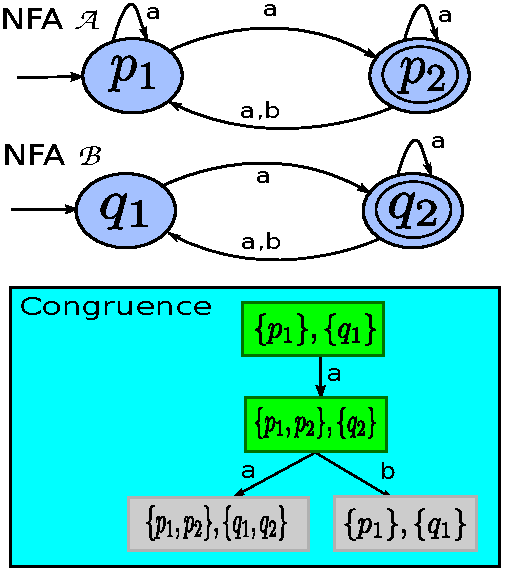
\includegraphics[scale=0.5]{fig/congr1.pdf}
		\hspace{0.55cm}
  	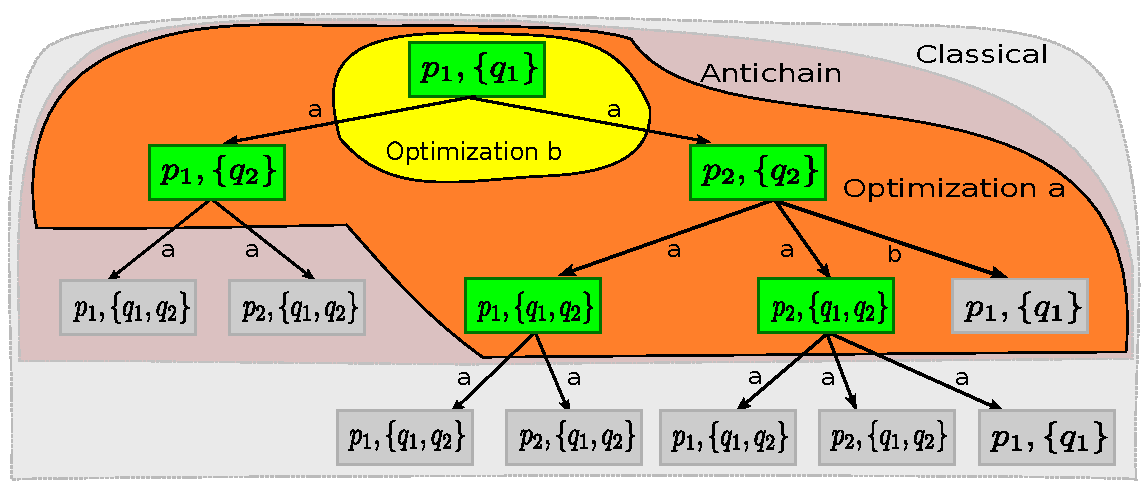
\includegraphics[scale=0.5]{fig/ac1.pdf}
	}
  \caption{
      \rm{
      \hspace{0.1cm} The picture is based on an example from \cite{tacas10}.
      It shows the procedure of checking language inclusion between two NFA using the mentioned approaches (which correspond to the labeled areas).
      %The labeled areas correspond to mentioned approaches.
      The antichain algorithm reduces number of the generated states compared with the classical,
      e.g., $(p_2,\{q_1,q_2\})$ is not further explored because $(p_2,\{q_2\}) \sqsubseteq (p_2,\{q_1,q_2\})$. 
      The optimization a and b are improvements of the antichain algorithm using simulation. 
      The congruence algorithm also reduces number of the generated states, so $(\{p_1,p_2\},\{q_1,q_2\})$ 
      is not further explored because it is in congruence closure 
      of the set of visited states.}}
      %It shows macrostates 
			%that are generated when checking language inclusion between two NFA using different approaches. Optimization a and b
			%correspond to the parts of the improvement of antichain algorithm using simulation.}}
  \label{automata}
\end{center}
\end{figure}



\chapter{Existing Finite Automata Libraries and the VATA Library} 
\label{libraries}
There are many different libraries for finite automata. These libraries have been created for various purposes and 
are implemented in different languages. 
At this chapter, some libraries will be described. Described libraries are just examples which represents typical disadvantages of existing libraries like
classical approach for language inclusion testing which needs determinisation of finite automaton. 

As the second VATA library for manipulating of \emph{tree} automata will be introduced. It will be briefly describe library design, operations for tree
automata and plans for extension of VATA library.

\section{Existing Finite Automata Libraries}
\label{existinglibraries}
\subsection{dk.brics.automaton}
\label{brics}
\emph{dk.brics.automaton} is an established Java package available under the BSD license. The latest version of this library (1.11-8) 
was released on September 7th, 2011.
Library can be downloaded and more information are on \cite{brics}. 

Library can use as input regular expression created by the Java \emph{RegeExp} class.
It supports manipulation with NFA and DFA. Basic operation like union,
intersection, complementation or run of automaton on the given word etc., are available.

Test of language inclusion is also supported but if the input automaton is NFA, it needs to be converted to DFA. 
This is made by \emph{subset construction} approach which is inefficient \cite{cav06}, \cite{tacas10}.

\emph{dk.brics.automaton} was ported to another two languages in two different libraries, which will be described next.

\subsubsection{libfa}
\emph{libfa} is a C library being part of \emph{Augeas} tool. 
Library is licensed under the LGPL, version 2 or later. It also support both versions of finite automata, NFA and DFA. 
Regular expressions could serve like input again.
libfa can be found and downloaded on \cite{libfa}.
libfa has no explicit operation for inclusion checking, but has the operations for intersection and complement of automata
which can serve for the inclusion checking.
Main disadvantage of libfa is again need of determinisation.

\subsubsection{Fare}
\emph{Fare} is a library, which brings dk.brics.automaton from Java to .NET. 
This library has the same characteristics as dk.brics.automaton or libfa and disadvantage in need of determinisation is still here. 
Fare can be found on \cite{fare}.

\subsection{The RWHT FSA toolkit}
The \emph{RWHT FSA} is a toolkit for manipulating finite automata described in \cite{kanthakN04}. 
The latest version is 0.9.4 from year 2005. The toolkit is written in C++
and available under its special license, derived from Q Public License v1.0 and the Qt Non-Commercial License v1.0. Library can be downloaded from \cite{rwth}. 

The RWHT FSA does not support only the classical finite automata, but also automata with weighted transitions so the toolkit has wider range of application.
The toolkit implements some techniques for better computation efficiency. E.g., it supports on-demand computation technique 
so not all computations are evaluated immediatelly but some are not computed until their results are really
needed. Usage of this technique leads to better memory efficiency. 

The RWHT FSA toolkit does not support language inclusion checking explicitly, but contains operations for intersection, complement and
determinisation which can be exploited for testing inclusion. This causes that the problem of a state explosion during 
the explicit determinization of an automaton is still here. 

\subsection{Implementation of New Efficient Algorithms}
There have been recently introduced some new efficient algorithms for inclusion checking 
which are dealing with problem of a state explosion because they avoid the explicit determinization of a finite automaton \cite{cav06,tacas10} and \cite{popl13}.
These state-of-the-art algorithms were implemented in OCaml languaue (mainly) for testing and evaluation purposes.

Some of the mentioned algorithms (\cite{cav06,taca10}) are possible to use not only for finite automat but also for tree automata. 
These algorithms for tree automata are provided by the VATA library which is implemented in C++ what brings the greater efficiency compared to OCaml implmentation. 
A description of this library will be placed in next section.
Despite the fact that a C++ implementation could be more efficient too, there is currently no library or toolkit similiar to VATA library providing 
these algorithms of inclusion checking for finite automata.


\begin{comment}
For finite automata manipulation exists many different libraries. Libraries have different purposes and are implemented in different languages, 
e.g. established package of Java \emph{dk.brics.automaton} \cite{brics}, \cite{tacas10}, which is also reimplemented for C in \emph{libfa} \cite{libfa} 
and for C\# in \emph{Fare} \cite{fare}. Another libraries are \emph{The RWTH FSA toolkit} \cite{rwth} in C++, which also supports weighted automata, or
\emph{FSA Utilities toolbox} \cite{fsaprolog} in Prolog.

This is not definitely complete enumeration of finite automata libraries, but just few examples. Their main problem is that they do not contain 
the efficient inclusion testing. On the other side, new efficient algorithms introduced in \cite{cav06,tacas10} and in \cite{popl13} have been for finite automata
implemented only in OCaml and implementation in C++ could be much more efficient.

Because of these reasons, algorithms for finite automata manipulation will be implemented as extension of VATA (library for tree automata manipulation) in C++.
\end{comment}

\section{VATA library}
\label{VATA}
\subsection{General}
VATA is a highly efficient open source library for manipulating \emph{non deterministic tree} automata licensed under GPL, version 3. 
Main application of VATA is in formal verification.
VATA library is implemented in C++ and uses the Boost C++ library. Download of library can be found on its website 
\footnote{\url{http://www.fit.vutbr.cz/research/groups/verifit/tools/libvata/}} \cite{libvata}.  

Purposes of VATA library are similar as purposes of this work and becasue VATA also provides basic infrastructure for 
parsing, serialing and writing finite automata from an input format, 
it was decided not to create a brand new library, but makes extension of VATA.
for finite automata.

\subsection{Design}
\label{sectionDesignVata}
VATA provides two kind of encoding for tree automata -- Explicit Encoding (top-down) and Semi-symbolic encoding (top-down and bottom-up). The main difference
between encoding is
in data structure for storing transition of \emph{tree} automata. Semi-symbolic encoding is primary for automata with large alphabets. 

The main idea of the desing of VATA library is show on the image \ref{picVataDesign}. Here is also brief description of that idea. 
The input automata are processed by one of the parsers (currently
here is only Timbuk format parser implemented). A result of parsing is a data structure with the information about automaton (it keeps the list
of transtion of given automaton, its final states etc.). The main progam choose one of the internal encodings of the automata. These encodings
contain a definiton of a data structure for a representation of automaton and fuctions which create transform the automaton from the data structure
created by parser to the data structure of chosen encoding. Each encoding also provide
an implementation of the operations over automata. 
Finally, once all needed operations over the input automata are processed, the result automaton can be dump to a output text format using one of serializers 
(currently there is only Timbuk format serializer implemented).

As you
can see on picture \ref{picVataDesign}, VATA is written in a modular way, so it is easy to make an extension for finite automata. Thanks to the modularity, 
any new encoding can share other parts of library such as parser or serializer \cite{libvata}. VATA also provides a command line interface which is shared by
different encodings.

\begin{figure}[h]
\begin{center}
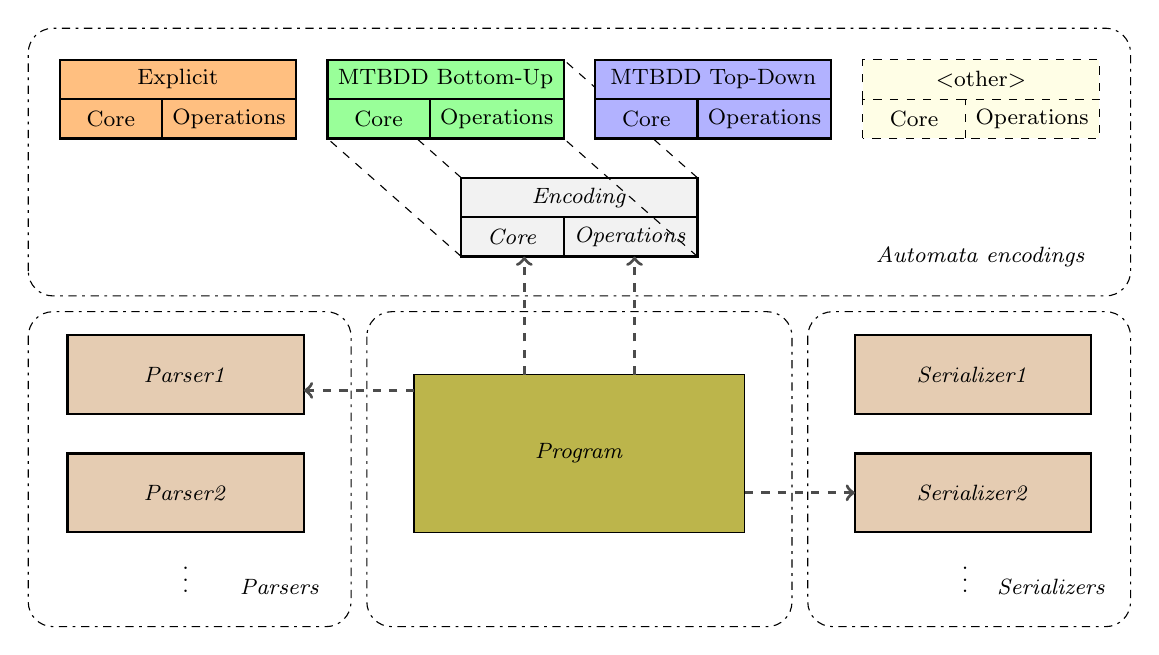
\begin{tikzpicture}
[
  scale=1,
  transform shape,
	gen/.style={thick,fill=gray!10},
	expl/.style={thick,fill=orange!50},
	bu/.style={thick,fill=green!40},
	td/.style={thick,fill=blue!30},
	other/.style={fill=yellow!10,dashed}
]
\tikzstyle{every node}=[font=\footnotesize]


% encodings
\draw[dashed] (0,1) -- (-1.7,2.5);
\draw[dashed] (0,0) -- (-1.7,1.5);
\draw[dashed] (3,1) -- (1.3,2.5);

\draw (0,0.5) rectangle +(3, 0.5) [gen] node[midway] {\textit{Encoding}};
\draw (0,0) rectangle +(1.3, 0.5) [gen] node[midway] {\textit{Core}};
\draw (1.3,0) rectangle +(1.7, 0.5) [gen] node[midway] {\textit{Operations}};

\draw (-5.1,2) rectangle +(3, 0.5) [expl] node[midway] {Explicit};
\draw (-5.1,1.5) rectangle +(1.3, 0.5) [expl] node[midway] {Core};
\draw (-3.8,1.5) rectangle +(1.7, 0.5) [expl] node[midway] {Operations};

\draw (-1.7,2) rectangle +(3, 0.5) [bu] node[midway] {MTBDD Bottom-Up};
\draw (-1.7,1.5) rectangle +(1.3, 0.5) [bu] node[midway] {Core};
\draw (-0.4,1.5) rectangle +(1.7, 0.5) [bu] node[midway] {Operations};

\draw (1.7,2) rectangle +(3, 0.5) [td] node[midway] {MTBDD Top-Down};
\draw (1.7,1.5) rectangle +(1.3, 0.5) [td] node[midway] {Core};
\draw (3.0,1.5) rectangle +(1.7, 0.5) [td] node[midway] {Operations};

\draw (5.1,2) rectangle +(3, 0.5) [other] node[midway] {$<$other$>$};
\draw (5.1,1.5) rectangle +(1.3, 0.5) [other] node[midway] {Core};
\draw (6.4,1.5) rectangle +(1.7, 0.5) [other] node[midway] {Operations};

\draw[dashed] (3,0) -- (1.3,1.5);

\draw[rounded corners=9,dash pattern=on 3pt off 2pt on 1pt off 2pt] (-5.5,-0.5) rectangle +(14,3.4);

\draw (6.6,0) node {\textit{Automata encodings}};


% parsers
\draw (-5,-2) rectangle +(3, 1) [gen,fill=brown!40] node[midway] (parser1) {\textit{Parser1}};
\draw (-5,-3.5) rectangle +(3, 1) [gen,fill=brown!40] node[midway] {\textit{Parser2}};
\draw (-3.5,-4) node {$\vdots$};

\draw[rounded corners=9,dash pattern=on 3pt off 2pt on 1pt off 2pt] (-5.5,-0.7) rectangle +(4.1,-4);
\draw (-2.3,-4.2) node {\textit{Parsers}};

% serializers
\draw (5,-2) rectangle +(3, 1) [gen,fill=brown!40] node[midway] {\textit{Serializer1}};
\draw (5,-3.5) rectangle +(3, 1) [gen,fill=brown!40] node[midway] {\textit{Serializer2}};
\draw (6.4,-4) node {$\vdots$};

\draw[rounded corners=9,dash pattern=on 3pt off 2pt on 1pt off 2pt] (4.4,-0.7) rectangle +(4.1,-4);
\draw (7.5,-4.2) node {\textit{Serializers}};

% program
\draw[rounded corners=9,dash pattern=on 3pt off 2pt on 1pt off 2pt] (-1.2,-0.7) rectangle +(5.4,-4);

\draw[fill=olive!60] (-0.6,-1.5) rectangle (3.6,-3.5) node[midway] {\textit{Program}};

\draw[very thick,dashed,->,black!70] (-0.6,-1.7) -- (-2,-1.7);
\draw[very thick,dashed,->,black!70] (3.6,-3) -- (5,-3);
\draw[very thick,dashed,->,black!70] (0.8,-1.5) -- (0.8,0);
\draw[very thick,dashed,->,black!70] (2.2,-1.5) -- (2.2,0);

\end{tikzpicture}

		\label{picVataDesign}
		\caption{The VATA library design. The image is taken from \cite{libvata}}.
\end{center}
\end{figure}

%%TODO: Vic se rozkecat o kodovanich
\subsubsection{Explicit Encoding}
\label{sectionExplicitEnc}
For storing explicit encoding top-down transitions (transitions are in form $q \xrightarrow{a} (q_1,...,q_n)$) 
is used \emph{hierarchical data structure based on hash tables}. First level of look-up
table maps the states to \emph{transition cluster}. This clusters are also look-up table and maps symbols of input alphabet
to the set of pointers (stored as \emph{red-black tree}) to tuples of states. Storing tuples of states is of course very memory demanding, so special
designed hash table was used for storing them. Inserting new transition to this structure requires a constant number of steps (exception is worst case scenario)
\cite{libvata}. This data structure can be seen on figure \ref{figExplicitTreeDataStr}.

\begin{figure}[h]
\begin{center}
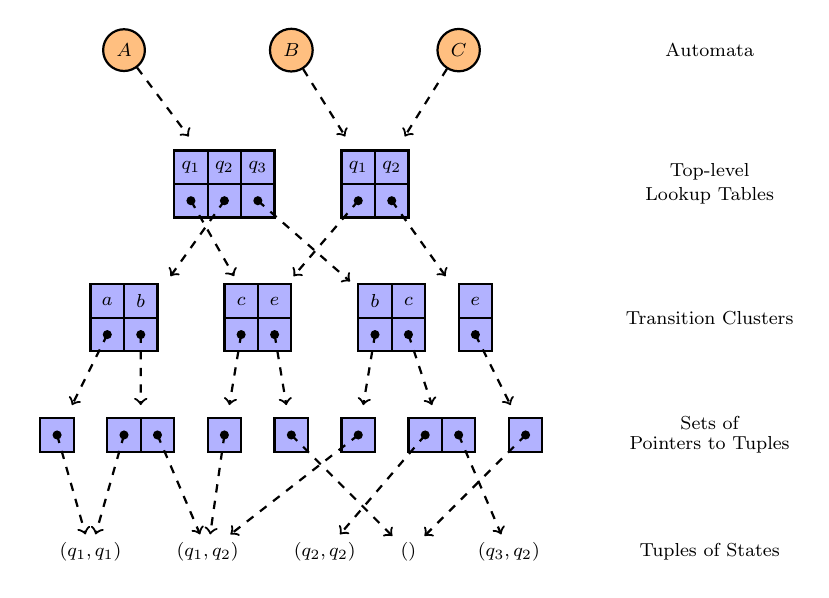
\begin{tikzpicture}
[
  scale=0.85,
  transform shape,
	gen/.style={thick,fill=gray!10},
	expl/.style={thick,fill=orange!50},
	bu/.style={thick,fill=green!40},
	td/.style={thick,fill=blue!30},
	other/.style={fill=yellow!10,dashed}
]

\node at(10,2) {Automata};

\node[expl,circle,draw] (aA) at(1.25,2) {\textit{$A$}};
\node[expl,circle,draw] (aB) at(3.75,2) {\textit{$B$}};
\node[expl,circle,draw] (aC) at(6.25,2) {\textit{$C$}};


\node at(10,0) {\shortstack{Top-level\\ Lookup Tables}};

\node[minimum size=40pt](table1) at (2.75,0) {};
\draw (2,0) rectangle +(0.5, .5) [td] node[midway] {\textit{$q_1$}};
\draw (2,-.5) rectangle +(0.5, .5) [td] node[midway] {};
\draw (2.5,0) rectangle +(0.5, .5) [td] node[midway] {\textit{$q_2$}};
\draw (2.5,-.5) rectangle +(0.5, .5) [td] node[midway] {};
\draw (3,0) rectangle +(0.5, .5) [td] node[midway] {\textit{$q_3$}};
\draw (3,-.5) rectangle +(0.5, .5) [td] node[midway] {};

\node[minimum size=40pt](table2) at (5,0) {};
\draw (4.5,0) rectangle +(0.5, .5) [td] node[midway] {\textit{$q_1$}};
\draw (4.5,-.5) rectangle +(0.5, .5) [td] node[midway] {};
\draw (5,0) rectangle +(0.5, .5) [td] node[midway] {\textit{$q_2$}};
\draw (5,-.5) rectangle +(0.5, .5) [td] node[midway] {};


\draw[->,thick,dashed] (aA) -- (table1);
\draw[->,thick,dashed] (aB) -- (table2);
\draw[->,thick,dashed] (aC) -- (table2);


\node at(10,-2) {Transition Clusters};

\node[minimum size=35](cluster1) at (1.5,-2) {};
\draw (0.75,-2) rectangle +(0.5, .5) [td] node[midway] {\textit{$a$}};
\draw (0.75,-2.5) rectangle +(0.5, .5) [td] node[midway] {};
\draw (1.25,-2) rectangle +(0.5, .5) [td] node[midway] {\textit{$b$}};
\draw (1.25,-2.5) rectangle +(0.5, .5) [td] node[midway] {};

\node[minimum size=35pt](cluster2) at (3.25,-2) {};
\draw (2.75,-2) rectangle +(0.5, .5) [td] node[midway] {\textit{$c$}};
\draw (2.75,-2.5) rectangle +(0.5, .5) [td] node[midway] {};
\draw (3.25,-2) rectangle +(0.5, .5) [td] node[midway] {\textit{$e$}};
\draw (3.25,-2.5) rectangle +(0.5, .5) [td] node[midway] {};

\node[minimum size=35pt](cluster3) at (5.25,-2) {};
\draw (4.75,-2) rectangle +(0.5, .5) [td] node[midway] {\textit{$b$}};
\draw (4.75,-2.5) rectangle +(0.5, .5) [td] node[midway] {};
\draw (5.25,-2) rectangle +(0.5, .5) [td] node[midway] {\textit{$c$}};
\draw (5.25,-2.5) rectangle +(0.5, .5) [td] node[midway] {};

\node[minimum size=35pt](cluster4) at (6.5,-2) {};
\draw (6.25,-2) rectangle +(0.5, .5) [td] node[midway] {\textit{$e$}};
\draw (6.25,-2.5) rectangle +(0.5, .5) [td] node[midway] {};


\draw[thick,fill=black] (2.25,-0.25) circle (0.5mm);
\draw[->,thick,dashed] (2.25,-.25) -- (cluster2);

\draw[thick,fill=black] (2.75,-0.25) circle (0.5mm);
\draw[->,thick,dashed] (2.75,-.25) -- (cluster1);

\draw[thick,fill=black] (3.25,-0.25) circle (0.5mm);
\draw[->,thick,dashed] (3.25,-.25) -- (cluster3);

\draw[thick,fill=black] (4.75,-0.25) circle (0.5mm);
\draw[->,thick,dashed] (4.75,-.25) -- (cluster2);

\draw[thick,fill=black] (5.25,-0.25) circle (0.5mm);
\draw[->,thick,dashed] (5.25,-.25) -- (cluster4);


\node at(10,-3.75) {\shortstack{Sets of\\ Pointers to Tuples}};

\node[minimum size=25pt](set1) at (0.25,-3.75) {};
\draw (0,-4) rectangle +(0.5, .5) [td] node[midway] {};

\node[minimum size=25pt](set2) at (1.5,-3.75) {};
\draw (1,-4) rectangle +(0.5, .5) [td] node[midway] {};
\draw (1.5,-4) rectangle +(0.5, .5) [td] node[midway] {};

\node[minimum size=25pt](set3) at (2.75,-3.75) {};
\draw (2.5,-4) rectangle +(0.5, .5) [td] node[midway] {};

\node[minimum size=25pt](set4) at (3.75,-3.75) {};
\draw (3.5,-4) rectangle +(0.5, .5) [td] node[midway] {};

\node[minimum size=25pt](set5) at (4.75,-3.75) {};
\draw (4.5,-4) rectangle +(0.5, .5) [td] node[midway] {};

\node[minimum size=25pt](set6) at (6,-3.75) {};
\draw (5.5,-4) rectangle +(0.5, .5) [td] node[midway] {};
\draw (6,-4) rectangle +(0.5, .5) [td] node[midway] {};

\node[minimum size=25pt](set7) at (7.25,-3.75) {};
\draw (7,-4) rectangle +(0.5, .5) [td] node[midway] {};


\draw[thick,fill=black] (1,-2.25) circle (0.5mm);
\draw[->,thick,dashed] (1,-2.25) -- (set1);

\draw[thick,fill=black] (1.5,-2.25) circle (0.5mm);
\draw[->,thick,dashed] (1.5,-2.25) -- (set2);

\draw[thick,fill=black] (3,-2.25) circle (0.5mm);
\draw[->,thick,dashed] (3,-2.25) -- (set3);

\draw[thick,fill=black] (3.5,-2.25) circle (0.5mm);
\draw[->,thick,dashed] (3.5,-2.25) -- (set4);

\draw[thick,fill=black] (5,-2.25) circle (0.5mm);
\draw[->,thick,dashed] (5,-2.25) -- (set5);

\draw[thick,fill=black] (5.5,-2.25) circle (0.5mm);
\draw[->,thick,dashed] (5.5,-2.25) -- (set6);

\draw[thick,fill=black] (6.5,-2.25) circle (0.5mm);
\draw[->,thick,dashed] (6.5,-2.25) -- (set7);


\node at(10,-5.5) {Tuples of States};

\node(tup1) at (0.75,-5.5) {$(q_1, q_1)$};
\node(tup2) at (2.5,-5.5) {$(q_1, q_2)$};
\node(tup3) at (4.25,-5.5) {$(q_2, q_2)$};
\node(tup4) at (7,-5.5) {$(q_3, q_2)$};
\node(tup5) at (5.5,-5.5) {$()$};

\draw[thick,fill=black] (0.25,-3.75) circle (0.5mm);
\draw[->,thick,dashed] (0.25,-3.75) -- (tup1);

\draw[thick,fill=black] (1.25,-3.75) circle (0.5mm);
\draw[->,thick,dashed] (1.25,-3.75) -- (tup1);

\draw[thick,fill=black] (1.75,-3.75) circle (0.5mm);
\draw[->,thick,dashed] (1.75,-3.75) -- (tup2);

\draw[thick,fill=black] (2.75,-3.75) circle (0.5mm);
\draw[->,thick,dashed] (2.75,-3.75) -- (tup2);

\draw[thick,fill=black] (3.75,-3.75) circle (0.5mm);
\draw[->,thick,dashed] (3.75,-3.75) -- (tup5);

\draw[thick,fill=black] (4.75,-3.75) circle (0.5mm);
\draw[->,thick,dashed] (4.75,-3.75) -- (tup2);

\draw[thick,fill=black] (5.75,-3.75) circle (0.5mm);
\draw[->,thick,dashed] (5.75,-3.75) -- (tup3);

\draw[thick,fill=black] (6.25,-3.75) circle (0.5mm);
\draw[->,thick,dashed] (6.25,-3.75) -- (tup4);

\draw[thick,fill=black] (7.25,-3.75) circle (0.5mm);
\draw[->,thick,dashed] (7.25,-3.75) -- (tup5);


\end{tikzpicture}

		\label{figExplicitTreeDataStr}
    \caption{The data structure for storing transtion of an tree automaton. There is a hash table (top-level lookup table) 
      which map a state to the pointer to another hash table (transition cluster). Transition cluster
      maps a symbols of input alphabet to the pointer to the set of pointers to the tuples.}
\end{center}
\end{figure}


For better performance is used \emph{copy-on-write} technique \cite{libvata}. The principle of this technique is, 
that on copy of automaton is created just new pointer to transition table of original automaton and after adding new state to one automaton (original or
copy) is modified only part of the shared transition table. 

\subsubsection{Semi-symbolic Encoding}
Transition functions in semi-symbolic encoding are stored in \emph{multi-terminal binary decision diagrams} (MTBDD), which are extension of \emph{binary decision 
diagrams}. There are provided top-down (transitions are in form $q \xrightarrow{a} (q_1,...,q_n)$, for $a$ with arity $n$) 
and bottom-up (transitions are in form $(q_1,...,q_n)\xrightarrow{a}q$) representation of tree automata in semi-symbolic encoding. 
The interesting part is saving of symbols in MTBDD. In top-down encoding, the input
symbols are stored in MTBDD with their arity, because we need to be able to distinguish between two instances of same symbols with different arity.
In opposite case, bottom-up encoding does not need to store arity, because it is possible to get it from arity of tuple on left side of transition \cite{libvata}.

For purposes of VATA library was implemented new MTBDD package, which improved the performance of library.

%TODO povypravaet o MTBDD package

\subsubsection{Operations}
There are supported basic operations over tree automata 
like union, intersection, elimination of unreachable states, but also some advance a algorithms for inclusion checking, 
computation of simulation relation, language preserving size reduction based on simulation equivalence. 

For inclusion testing are implemented optimized algorithms from \cite{cav06,tacas10}. The inclusion operation is implemented in more versions, so it is possible
to use only some heuristic and compare different results.

Efficiency of advanced operations does not come only from the usage of efficient algorithms, 
but there are also some implementation optimization like \emph{copy-on-write}
principle for automata copying (briefly described in subsection \ref{sectionExplicitEnc}), buffering once computed clusters of transitions etc. 
Other optimization could be found in exploitation of polymorphism using C++ function templates, instead of
virtual method because call of virtual function leads to indirect functions call using look-up virtual-method table (because compiler does not know, which 
function will be called in runtime) what brings an overhead comapred to classical direct
function call and it also precludes compiler's optimizer to perform some operations \cite{libvata}. 
%TODO Moznost citatce 

More details about implementation optimization can be found in \cite{libvata}.

Especially advanced operations are able only for specific encoding. Some of operations implemented in VATA library and their supported encodings are in this table:
\begin{savenotes}
\begin{table}[h]
	\begin{center}
		\catcode`\-=12
		\begin{tabular}{| l | c | c | c |} \hline
		& {\textbf{Explicit}} & \multicolumn{2}{|c|}{\textbf{Semi-symbolic}} \\ \cline{2-4}
		\textbf{Operation} & \textbf{top-down} & \textbf{bottom-up} & \textbf{top-down} \\ \hline
		Union & $+$ & $+$ & $+$ \\
		Intersection & $+$ & $+$ & $+$ \\
		Complement & $+$ & $+$ & $+$ \\
		Removing useless states & $+$ & $+$ & $+$ \\
		Removing unreachable states & $+$ & $+$ & $+$ \\
		Downward and Upward Simulation & $+$ & $-$ & $+$ \\
		Bottom-Up Inclusion  & $+$ & $+$ & $-$ \\ 
		Simulation over LTS\footnote{LTS -- Labeled Transitions System} & $+$ & $-$ & $-$ \\ \hline
		\end{tabular}
	\caption{Table of some supported operations}
	\label{tab1}
	\end{center}
\end{table}
\end{savenotes}


\subsection{Extension for Finite Automata}
The main goal of this work is to 
provide operation for language inclusion test of
NFA without the need of explicit determinisation. To be precise, VATA library could be already used for finite automata, 
which can be represented like one dimensional
tree automata. But the VATA library data structures for manipulating tree automata are designated for more complex data structures
and new special implementation for finite
automata will be definitely more efficient. Not only inclusion checking algorithm will be implemented but also the algoritms for basic operations like
such as union, intersection, removing unreachable or useless states etc.
This new extension will use the explicit encoding for representing an automaton. 
The extension will use some already implemented features of VATA like parsing and serializing
the input automata or computation of simulation over states of an automaton.

\chapter{Design}
\label{design}
In this chapter will be described design of the newly created extension of VATA library for finite automata. 
Firstly, the data structures used for storing a finite automaton will be explain, then principle of translation of the states and the symbols to internal
representation and finally chosen input format and its modification.

\section{Data Structures for Explicit Encoding of Finite Automata}
\label{data structure explicit}
\subsection{Analysis}
\label{analysis}
An NFA is defined by set of its states, its start and final states (which are subset of all states of a NFA) and also its
transitions \ref{defNFA} and the input alphabet. One needs to keep information about sets of start and final states to be able to distinguish
between a start or a final state and the other states. But it is not neccessary to store the whole set of states because states that are not start or final
are used within transitions. This fact also hold in case of input alphabet. 

The set of transitions keeps the most information about an NFA and is also often used
during operations over NFA, so the the performance of these operations hardly depend on the efficiency of data structure for a set of transitions. For example,
one often wants to get all transitions for given state or for given state and given alphabet symbol. The similiar situaion is in the case
of tree automata when it is not neccessary to hold the whole set of state but it is important to have efficient data structure for represanting 
transitions of a given tree automata.

The data structure used for storing transions of a tree automaton in VATA library was described earlier \ref{sectionExplicitEnc} and can be seen
on the figure \ref{figExplicitTreeDataStr}. The evaluation of VATA library \cite{libvata} proves efficiency of this data structure is efficient, so it was
decided to modificate this data structure and use it also for part of VATA library for finite automata.

\subsection{Design of Data Structure for Transtions of NFA}
Data structure for storing transitions of an NFA is based on hash tables. The first hash table (top-level hash table) maps a given state to the pointer to
the transition cluster. The transition cluster is another hash table which maps a symbol of the input alphabet to a set of states. Described data structure is on
the figure \ref{figExplicitFADataStr}.

The data structure for finite automata transitions is simplyfication of the data structure for tree automata what is can be seen by comparing figures 
\ref{figExplicitFADataStr} and \ref{figExplicitTreeDataStr}. This simplyfication is possible because the tree version has to stored to whole tuples of
states in transtions. Since these tuple can be very large it is more efficient to store them only once and in data structure keeps pointer to the 
tuple, which is in a transtion, instead of the tuple alone. 
In case of finite automata this advantage dissapears because there are no tuples of state but only states alone and keeping pointer to one state will not 
bring any memory efficiency (the size of a pointer to a state and the state alone is quite similiar). This fact causes that in the data structure 
for finite automata is not needed to use anything like set of pointers to tuples in tree automata version, but could be directly used the set of states. This 
set of states would be pointed from transition cluster and would contain all states accessible from a given state under a symbol of input alphabet.

But there is possible another simplyfication. The set of states does not need to be in special level of data structure but can be integrated to the transition
cluster. When this optimization is applied, transition cluster maps symbol directly to the set of states accessible under this symbol.

The mentioned optimization enables that the tree version of data structure, which has four leves, was simplyfied to the two level data structure what brings
simplyier and more efficient manipulation with these data structure.

This data structure also aplly the copy-on-write principle, what brings better memory efficiency. It means that the look-up tables and 
the transtion clusters are shared among NFA when they are same and
a new look-up table and a transition is created only when a new item is inserted to the one of the automata.

Let give the examples for searching and inserting a trasition to this data structure for the NFA on the figure \ref{figExplicitFADataStr}. 
If one wants to find all accessibale states for state $q_1$ and symbol $a$ in a NFA $A$
so in the top-level lookup is found pointer to transition cluster for state $p$. In this
transition cluster is symbol $a$ mapped to the set of states (in this case ($\{q_1,q_2\}$)) which are accessible from $q_1$ under $a$.
If one wants to insert a new transition $q_3\rightarrow{e}q_2$ to a NFA $C$, the look-up table pointed by automaton $C$ is duplicated 
and a state $q_3$ is inserted to it. A NFA $C$ now points to that newly duplicated look-up table. State $q_3$ is mapped to pointer to the newly created
transition cluster. Symbol $e$ is inserted to this new transition cluster and mapped to the set of state which contains just state $q_2$.

\begin{figure}[h]
\begin{center}
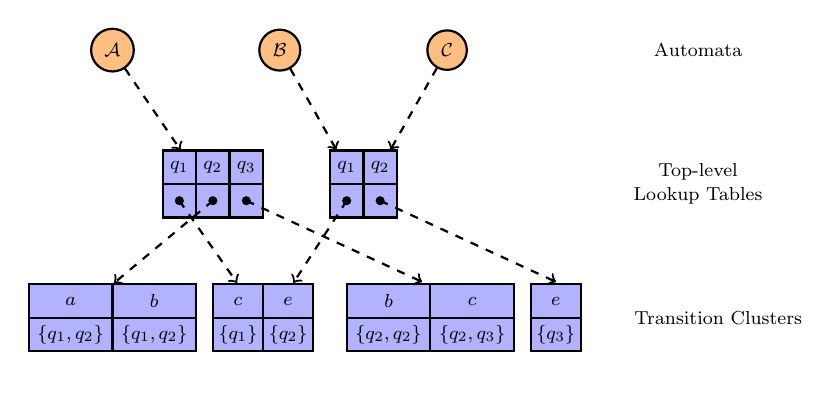
\begin{tikzpicture}
[
  scale=0.85,
  transform shape,
	gen/.style={thick,fill=gray!10},
	expl/.style={thick,fill=orange!50},
	bu/.style={thick,fill=green!40},
	td/.style={thick,fill=blue!30},
	other/.style={fill=yellow!10,dashed}
]

\node at(10,2) {Automata};

\node[expl,circle,draw] (aA) at(1.25,2) {\textit{$\mathcal{A}$}};
\node[expl,circle,draw] (aB) at(3.75,2) {\textit{$\mathcal{B}$}};
\node[expl,circle,draw] (aC) at(6.25,2) {\textit{$\mathcal{C}$}};


\node at(10,0) {\shortstack{Top-level\\ Lookup Tables}};

\node[minimum size=40pt](table1) at (2.75,-0.2) {};
\draw (2,0) rectangle +(0.5, .5) [td] node[midway] {\textit{$q_1$}};
\draw (2,-.5) rectangle +(0.5, .5) [td] node[midway] {};
\draw (2.5,0) rectangle +(0.5, .5) [td] node[midway] {\textit{$q_2$}};
\draw (2.5,-.5) rectangle +(0.5, .5) [td] node[midway] {};
\draw (3,0) rectangle +(0.5, .5) [td] node[midway] {\textit{$q_3$}};
\draw (3,-.5) rectangle +(0.5, .5) [td] node[midway] {};

\node[minimum size=40pt](table2) at (5,-0.2) {};
\draw (4.5,0) rectangle +(0.5, .5) [td] node[midway] {\textit{$q_1$}};
\draw (4.5,-.5) rectangle +(0.5, .5) [td] node[midway] {};
\draw (5,0) rectangle +(0.5, .5) [td] node[midway] {\textit{$q_2$}};
\draw (5,-.5) rectangle +(0.5, .5) [td] node[midway] {};


\draw[->,thick,dashed] (aA) -- (table1);
\draw[->,thick,dashed] (aB) -- (table2);
\draw[->,thick,dashed] (aC) -- (table2);


\node at(10.3,-2) {Transition Clusters};

\node[minimum size=35](cluster1) at (0.65,-2) {};
\draw (0.00,-2) rectangle +(1.25, .5) [td] node[midway] {\textit{$a$}};
\draw (0.00,-2.5) rectangle +(1.25, .5) [td] node[midway] {\textit{$\{q_1,q_2\}$}};
\draw (1.25,-2) rectangle +(1.25, .5) [td] node[midway] {\textit{$b$}};
\draw (1.25,-2.5) rectangle +(1.25, .5) [td] node[midway] {\textit{$\{q_1,q_2\}$}};

\node[minimum size=35pt](cluster2) at (3.55,-2.1) {};
\draw (2.75,-2) rectangle +(0.75, .5) [td] node[midway] {\textit{$c$}};
\draw (2.75,-2.5) rectangle +(0.75, .5) [td] node[midway] {\textit{$\{q_1\}$}};
\draw (3.5,-2) rectangle +(0.75, .5) [td] node[midway] {\textit{$e$}};
\draw (3.5,-2.5) rectangle +(0.75, .5) [td] node[midway] {\textit{$\{q_2\}$}};

\node[minimum size=35pt](cluster3) at (6.5,-1.75) {};
\draw (4.75,-2) rectangle +(1.25, .5) [td] node[midway] {\textit{$b$}};
\draw (4.75,-2.5) rectangle +(1.25, .5) [td] node[midway] {\textit{$\{q_2,q_2\}$}};
\draw (6.0,-2) rectangle +(1.25, .5) [td] node[midway] {\textit{$c$}};
\draw (6.0,-2.5) rectangle +(1.25, .5) [td] node[midway] {\textit{$\{q_2,q_3\}$}};

\node[minimum size=35pt](cluster4) at (8.5,-1.75) {};
\draw (7.5,-2) rectangle +(0.75, .5) [td] node[midway] {\textit{$e$}};
\draw (7.5,-2.5) rectangle +(0.75, .5) [td] node[midway] {\textit{$\{q_3\}$}};


\draw[thick,fill=black] (2.25,-0.25) circle (0.5mm);
\draw[->,thick,dashed] (2.25,-.25) -- (cluster2);

\draw[thick,fill=black] (2.75,-0.25) circle (0.5mm);
\draw[->,thick,dashed] (2.75,-.25) -- (cluster1);

\draw[thick,fill=black] (3.25,-0.25) circle (0.5mm);
\draw[->,thick,dashed] (3.25,-.25) -- (cluster3);

\draw[thick,fill=black] (4.75,-0.25) circle (0.5mm);
\draw[->,thick,dashed] (4.75,-.25) -- (cluster2);

\draw[thick,fill=black] (5.25,-0.25) circle (0.5mm);
\draw[->,thick,dashed] (5.25,-.25) -- (cluster4);
\end{tikzpicture}

		\label{figExplicitFADataStr}
    \caption{The data structure for storing transtion of an finite automaton. There is a hash table (top-level lookup table) 
      which map a state of a FA to the pointer to another hash table (transition cluster). Transition cluster maps a symbol of the input alphabet
      to a set of states.}
\end{center}
\end{figure}

\section{Start and final states data structure}
As it was mentioned before \ref{analysis} it is neccessary to keep start and final states in the special sets to be able distinguish between them and the others
states of an automaton. This is also main usage of these sets during operations over finite automata so there is no need to create special data structure and 
unordered set is efficient enough for them.

\section{Translation of the states and symbols}
The input automaton is is parsed and converted to intern representation. During this conversion to the intern representation are states translated
(mapped) from input type (e.g., text description of an automaton) 
to an integers and this also works for symbols of the input alphabet (principle can be seen on figure \ref{figExplicitFADataStr}). 
This mechanism brings better efficiency for manipulation with states and symbols
during the operations. It also provides unification all input forms to the one internal representation. 

The translated integeres can be changed during some operations (e.g., union) over finite automata but the relation between mapping and mapped value will
not be broken.

When the input automaton is processed by VATA library operations it is often serialized back to the input format. The result 
automaton's states are converted back to the input format from internal enconding using translation in reverse order
so the result notation stays consistent with the input.

\begin{figure}
\begin{center}
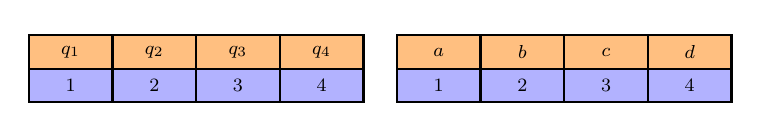
\begin{tikzpicture}
[
  scale=0.85,
  transform shape,
	gen/.style={thick,fill=gray!10},
	expl/.style={thick,fill=orange!50},
	bu/.style={thick,fill=green!40},
	td/.style={thick,fill=blue!30},
	other/.style={fill=yellow!10,dashed}
]

\node[minimum size=35](states) at (0.65,-2) {};
\draw (0.00,-2) rectangle +(1.25, .5) [expl] node[midway] {\textit{$q_1$}};
\draw (0.00,-2.5) rectangle +(1.25, .5) [td] node[midway] {\textit{$1$}};
\draw (1.25,-2) rectangle +(1.25, .5) [expl] node[midway] {\textit{$q_2$}};
\draw (1.25,-2.5) rectangle +(1.25, .5) [td] node[midway] {\textit{$2$}};
\draw (2.5,-2) rectangle +(1.25, .5) [expl] node[midway] {\textit{$q_3$}};
\draw (2.5,-2.5) rectangle +(1.25, .5) [td] node[midway] {\textit{$3$}};
\draw (3.75,-2) rectangle +(1.25, .5) [expl] node[midway] {\textit{$q_4$}};
\draw (3.75,-2.5) rectangle +(1.25, .5) [td] node[midway] {\textit{$4$}};

\node[minimum size=35](syms) at (0.65,-2) {};
\draw (5.5,-2) rectangle +(1.25, .5) [expl] node[midway] {\textit{$a$}};
\draw (5.5,-2.5) rectangle +(1.25, .5) [td] node[midway] {\textit{$1$}};
\draw (6.75,-2) rectangle +(1.25, .5) [expl] node[midway] {\textit{$b$}};
\draw (6.75,-2.5) rectangle +(1.25, .5) [td] node[midway] {\textit{$2$}};
\draw (8.0,-2) rectangle +(1.25, .5) [expl] node[midway] {\textit{$c$}};
\draw (8.0,-2.5) rectangle +(1.25, .5) [td] node[midway] {\textit{$3$}};
\draw (9.25,-2) rectangle +(1.25, .5) [expl] node[midway] {\textit{$d$}};
\draw (9.25,-2.5) rectangle +(1.25, .5) [td] node[midway] {\textit{$4$}};

\end{tikzpicture}

		\label{figExplicitFADataStr}
    \caption{Translator takes the input format (text format in this case) and maps it to the integer. On the figure can
    be seen mapping symbols (on the left) and mapping input symbols (on the right).}
\end{center}
\end{figure}

\section{Usage of the Timbuk format}
\label{usageTimub}
Because there is no standard format for describing the finite automato, the Timbuk format \cite{timbuk} was chosen as input and output text format
of the finite automata. The timbuk format is also used as an format for tree automata in VATA library. 
In fact, the original purpose of the Timbuk format is describing tree automata but with some modifications can be used also for finite automata. 
Here is an example of a finite automaton in the Timbuk format:\\
\texttt {
  \textbf{Ops} $a:1$ $x:0$\\
  \textbf{Automaton} example\\
  \textbf{States} $s$ $p$ $q$ $f$\\
  \textbf{Final States} $f$\\
  \textbf{Transitions}\\
  \indent $x \rightarrow s$\\
  \indent $a(s) \rightarrow p$\\
  \indent $a(s) \rightarrow q$\\
  \indent $a(p) \rightarrow f$\\
  \indent $a(q) \rightarrow f$\\
}
On the first line of the specification in the Timbuk format
is specified that the automaton has only one symbol of the input alphabet $a$ with arity one (arity of the symbols of finita automata will
be always one). 
The need of specification of the arity of an input symbol is
lack which comes from the original purpose of the timbuk format because it is necessary to give the arity of an symbol of the input alphabet of an tree automaton.

The second symbol $x$ with arity zero is not actually symbol of the input alphabet but is used for definition of the start states. The
start states are defined in section \emph{Transitions} by the transitions which has on the left side some symbol with zero symbol and on the
right side of the transiton is a start state. This is again disadvantage
of the Timbuk format because in the case of tree automata there are defined no start states.

On the second line of the given example specification in the Timbuk format is name of the automaton (in our case is the name \emph{example}). 
On the third line is a list of states of the automaton and on the fourth line is a list of final states of the automaton.

Then there is list of the transitions of the automaton. 
For example, the transition $s \xrightarrow{a} q$ is in the Timbuk format described like $a(s)\rightarrow q$.

\section{Overview of used interfaces of VATA library}
The new extension of VATA library has not been built from scratch but uses some parts of the existing library and here is give their list.

\subsubsection{Parser and Serializer}
Because for finite automata have been used the same input and output format \ref{usageTimbuk} it possible to use the original parse and serializer for this 
format which have been implemented in the existing part of library. 
The parser returns a data structure which generally describes a finite automaton and this data structure is futher processed in part of library for 
finite automata where is converted to the data structure for explicit encoding of the finite automata. When one wants to dump an automaton from explicit encoding
back to the text format, the automaton is converted to a data structure which is identical with a data structure returned by parser. 
Description of an automaton in this
data structure is given to the serializer which dumps it to the text format.

\subsubsection{Simulation}
One of the operations over finite automata, which VATA provides, is computing simulation of an automaton. For computation of the simulation relation
is possible to use the existing implementation of this operation. 
The difference is in the conversion of an finite automaton into the Labeled Transition System (LTS) which
needs to be implemented in part of library for finite automata.

\subsubsection{Utilities}
The original VATA library also provides lot of utilities which are also usefull for implementation of extension for the finite automata. These utilities
provides classes for easier processing of finite automata. For example, the classes \emph{TwoWayDict} and \emph{TranslatorStrict} are uses for conversion
of an finite automaton to the explicit encoding, the class \emph{Antichain2Cv2} is used for storing states to the antichain during checking inclusion using
antichain algorithm \ref{sectionAntichain} and the class \emph{AutDescription} for represanting an automaton after the parsing.

The usage of the of this utilies speeds up the development of the module for finite automata and also keeps the library more compact because no
redundat code is produced.

\chapter{Implementation}
\label{implementation}
\section{implementation of basic operations}
\section{implementation of antichain algorithms}
\section{improvments for simulation}
\section{implementation of congruence closure}

\chapter{Experimental evaluation}
\label{eval}
\section{improvemnet give by congrunce}

\chapter{Conclusion}
\label{concl}
\section{futher development}
